\documentclass[11pt]{article}

\usepackage[utf8]{inputenc}
\usepackage[T1]{fontenc}
\usepackage{amsmath}
\usepackage{amssymb}
\usepackage{booktabs}
\usepackage{graphicx}
\usepackage[numbers]{natbib}
\usepackage{hyperref}
\usepackage{geometry}
\geometry{margin=1in}

\title{One Small Network versus an Ensemble for Predicting Allelic Skew in Reporter Assays: A Blind Evaluation}
\author{[Authors to be added]}
\date{}

\begin{document}
\maketitle

\begin{abstract}
Massively parallel reporter assays (MPRAs) measure the regulatory activity of hundreds of thousands of DNA pieces; their allelic form measures how a single-letter change alters activity (allelic skew). The strongest published predictor of skew on a large plasmid-MPRA natural-variant table, MPAC, averages 10 networks of about 4.1M parameters for each chromosome; small single networks were trained on a different assay. We train one 1.32M-parameter network, the published MPRA-LegNet design with a body shared by 8 outputs spanning lentiviral and plasmid MPRAs, plus self-distillation, and fixed it and four pass marks before scoring three locked chromosomes once. On 29,397 locked variants, our model (model 2) reached an effect Pearson (correlation of predicted with measured skew) of 0.594, against 0.508 for the same design trained on lentiviral MPRA only (difference 0.086, 95\% interval 0.074 to 0.099) and 0.466 for the published MPRA-LegNet; part of this gain is a same-assay advantage. Model 2 was slightly but significantly behind MPAC (0.604; difference $-0.010$, 95\% interval $-0.019$ to $-0.001$), which we ran with one window instead of its published 18. On practice chromosomes a single MPAC network matched model 2 (0.583 against 0.584), so the ensemble's lead comes from averaging; averaging all 10 of our models, which agree more with each other, reached only 0.589. Self-distillation added about 0.011; of eight other changes screened, only a wider body helped. A leak-guard flaw found after the test changed the main result by 0.004. Weights and a prediction script will be released.
\end{abstract}

\section{Introduction}
Most variants associated with human traits lie in non-coding regulatory DNA, where their effects are hard to read from sequence alone \cite{siraj2026functional}. Massively parallel reporter assays (MPRAs) address this experimentally: each of hundreds of thousands of short DNA pieces is placed next to a reporter gene with a unique barcode, and the ratio of reporter RNA to DNA counts, usually reported as a log2 fold change (log2FC), measures the piece's regulatory activity \cite{melnikov2012systematic,patwardhan2012massively,inoue2015decoding}. In the allelic form of the assay, the two versions of a piece that differ at one letter are measured side by side, and the log2 ratio of their activities, the allelic skew, measures the variant's effect \cite{tewhey2016direct,ulirsch2016systematic,siraj2026functional}. Reporters can be carried on plasmids or, in lentiviral MPRA (lentiMPRA), integrated into the genome \cite{gordon2020lentimpra,agarwal2025massively}; saturation mutagenesis measures every single-letter change of an element \cite{kircher2019saturation}. Because no assay can test every variant, sequence-to-activity models trained on these data score variants that were never measured \cite{eraslan2019deep,zhou2015predicting,kelley2016basset}.

Two limits make it unclear how good a small model can be for this task. First, the published small network for human MPRA data, MPRA-LegNet, which uses the LegNet design \cite{penzar2023legnet}, was trained on lentiMPRA \cite{agarwal2025massively}, while a large table of measured allelic skews comes from a plasmid MPRA of fine-mapped trait variants \cite{siraj2026functional}. A model trained on one assay type learns that assay's notion of activity, so its effect predictions on the other assay may start at a disadvantage. Second, the strongest published predictor of skew on that table, MPAC \cite{butts2025identifying}, is an ensemble of Malinois networks \cite{gosai2024machineguided}: for any one chromosome it averages 10 networks of about 4.1M parameters. Skew is a small difference between predictions for two almost identical sequences, so a network's errors enter the effect directly; we hypothesised that averaging members whose errors differ cancels part of them. Whether the ensemble's lead reflects a better network or the averaging itself was not known. Finally, differences of 0.01 in correlation are hard to trust when the test set has informed model choices.

We ask how close one small network can get to the ensemble under a strictly blind evaluation, and what closes the gap. Keeping the published MPRA-LegNet design and recipe, we train one shared body with 8 outputs on two MPRA assay types at once: lentiMPRA in three cell lines and plasmid MPRA in five. Each row trains only the outputs in which it was measured, so the two assays share sequence features without mixing labels. We then add self-distillation from the average of three independently trained models of the same design \cite{hinton2015distilling,furlanello2018born}. We split the plasmid-MPRA table by chromosome before training, made every choice on practice chromosomes, and wrote down four pass marks before three locked chromosomes were scored once.

We call the resulting network model 2, and the same design trained on lentiMPRA only model 1. Our contributions are:
\begin{itemize}
\item a 1.32M-parameter network covering two MPRA assay types and 8 outputs, which reaches an effect Pearson of 0.594 on blind chromosomes, slightly but significantly behind a roughly 41M-parameter ensemble (0.604) and far ahead of the published small model (0.466), partly through a same-assay advantage;
\item a blind evaluation protocol (pre-declared marks, one-shot locked chromosomes, genome-block bootstrap, near-copy leak guards), with a disclosed leak-guard correction;
\item a measured decomposition of the gap to the ensemble: its single members match our single network (0.583 against 0.584 on practice chromosomes), and its lead comes from averaging members that agree less with each other than ours do;
\item negative results: of eight training and design changes screened, only a wider body helped.
\end{itemize}

\section{Related Work}
\paragraph{Models trained on reporter-assay data.} Convolutional networks fitted to reporter measurements predict activity from short sequences, for example DeepSTARR for STARR-seq enhancer activity \cite{almeida2022deepstarr}, models of random yeast promoter libraries \cite{vaishnav2022evolution}, and the entries of a community challenge that compared architectures and training strategies \cite{rafi2024community}. LegNet, an EfficientNetV2-inspired network, won that challenge and also predicts single-letter variant effects \cite{penzar2023legnet}; its lentiMPRA version, MPRA-LegNet, was trained on lentiMPRA in HepG2, K562 and WTC11 \cite{agarwal2025massively}. Malinois models MPRA activity in three cell types and was used to design cell-type-specific elements \cite{gosai2024machineguided}, and MPAC applies ensembles of Malinois networks to score non-coding variants at scale \cite{butts2025identifying}. A retrainable framework trained on whole-genome STARR-seq has been proposed for prioritizing variants that were not measured \cite{venukuttan2026modeling}. Each of these models was trained on one assay type; we train the LegNet design on two at once and measure the remaining gap to the ensemble blind.

\paragraph{Genome-scale models and variant scores.} Models trained on genome-wide functional tracks predict regulatory activity from longer sequences: DeepSEA and Basset \cite{zhou2015predicting,kelley2016basset}, Enformer \cite{avsec2021effective}, Borzoi \cite{linder2025predicting} and AlphaGenome \cite{avsec2026advancing}. Evaluations have examined their prediction of epigenomic profiles \cite{toneyan2022evaluating}, and found that they mostly ignore distal enhancers \cite{karollus2023current} and explain expression differences between individuals poorly \cite{sasse2023benchmarking}. A standardized comparison of models on enhancer variant effects from MPRA, raQTL and eQTL data found that CNN models performed best for predicting regulatory impact \cite{manzo2025comparative}. For disease variants, integrative and conservation-based scores such as CADD \cite{kircher2014general,rentzsch2018cadd} and phylogenetic language models such as PhyloGPN \cite{albors2025phylogenetic} are strong, and TraitGym benchmarks them on causal regulatory variants \cite{benegas2025benchmarking}. These models target labels other than reporter-assay skew; none of them was used to train or evaluate our models, and we use TraitGym only to bound our model's scope.

\paragraph{Augmentation, ensembling and distillation.} Deep ensembles improve predictive uncertainty estimates \cite{lakshminarayanan2016simple}, at a cost that grows with the number of members. Knowledge distillation trains one network to match the outputs of others \cite{hinton2015distilling}, and a student parameterized identically to its teacher can outperform it \cite{furlanello2018born}. In regulatory genomics, DEGU distils an ensemble into a single model that captures both the ensemble's mean and its variability \cite{zhou2026uncertaintyaware}, and EvoAug improves generalization with evolution-inspired sequence augmentations followed by fine-tuning on the original data \cite{lee2023evoaug}. Closest to our setting, Wang et al.\ \cite{wang2026synthetic} trained 16 chromosome-fold teachers on 110,359 K562 lentiMPRA elements, distilled them into one network, and used its predictions for 600,000 in-silico single-nucleotide substitutions to fine-tune Borzoi; they report that ensembling raised mean teacher Pearson $r$ from 0.32 to 0.34 on CAGI5 and from 0.54 to 0.57 on the Siraj et al.\ saturation-mutagenesis set, and that their distilled student reached 0.38 and 0.59 respectively, ahead of MPRA-LegNet (0.33) on CAGI5. Their teachers are fine-tuned AlphaGenome encoders and their evaluation is a different split and variant set, so their numbers are not comparable with ours; we note the agreement that a modest part of an ensemble's accuracy transfers to one network. We test self-distillation and EvoAug-style augmentation, and measure how much of an ensemble's lead a single member already has.

\section{Methods}
\label{sec:methods}

\subsection{Data}
\label{sec:data}

\paragraph{Lentiviral MPRA.} We used lentiMPRA activity tables from three cell lines \cite{agarwal2025massively}: HepG2 (61,463 elements), K562 (98,332 elements) and WTC11 (23,123 elements). Each row is a 200-letter regulatory piece between two 15-letter adapters (230 letters). Dataset folds 1 to 8 were used for training, fold 9 for validation (checkpoint choice) and fold 10 as a held-out test. Rows that were exact reverse-complement duplicates of other rows were dropped.

\paragraph{Plasmid MPRA natural-variant table.} The table of \citet{siraj2026functional} contains 304,278 variants, each with two 200-letter versions (reference and alternative allele) measured in HepG2, K562 and SK-N-SH (about 302,000 each), HCT116 (185,108) and A549 (125,796). We used only single-letter variants with two 200-letter versions (281,325). The table's coordinates are hg19. For a variant, the measured allelic skew is the log2 ratio of the activities of the alternative and reference versions.

\paragraph{Saturation-mutagenesis sets.} From the same plasmid MPRA study we used a saturation scan of 114 single-variant pieces, each in both allele backgrounds, with all 600 single-letter changes measured in HepG2 and K562. Before any scoring it was split into a practice half (odd chromosomes and X, 58 pieces) and a locked half (even chromosomes, 56 pieces); only backgrounds with baseline log2FC at least 1 were scored. We also used saturation mutagenesis of four regulatory elements (F9, LDLR, SORT1 and PKLR at 48 hours) from an earlier study \cite{kircher2019saturation}.

\paragraph{Out-of-scope check.} TraitGym Mendelian \cite{benegas2025benchmarking} (338 disease variants, 3,042 matched controls) was scored zero-shot, with CADD \cite{kircher2014general,rentzsch2018cadd} and PhyloGPN \cite{albors2025phylogenetic} as reference points.

\subsection{Split and leak guards}
\label{sec:split}

The natural-variant table was split by chromosome before any training (Figure~\ref{fig:schematic}b): locked test chromosomes 5, 14 and 22 (29,397 variants), practice chromosomes 6, 13 and 20 (28,104 variants), and training on all other chromosomes (208,783 variants, two pieces each). All modelling choices were made on the practice chromosomes, the saturation-scan practice half and lentiMPRA fold 9. Variants within 200 letters of a saturation-scan test piece were removed from training, and lentiMPRA pieces overlapping held-out variant pieces were removed. A near-copy guard compared 24-letter words: a training piece counts as a near-copy of a held-out piece, and is removed, if it shares at least 27 of its 177 24-letter words with any one held-out piece. Section~\ref{sec:leak} reports a flaw in our first implementation of this guard, found after the locked test.

\begin{figure}[htbp]
\centering
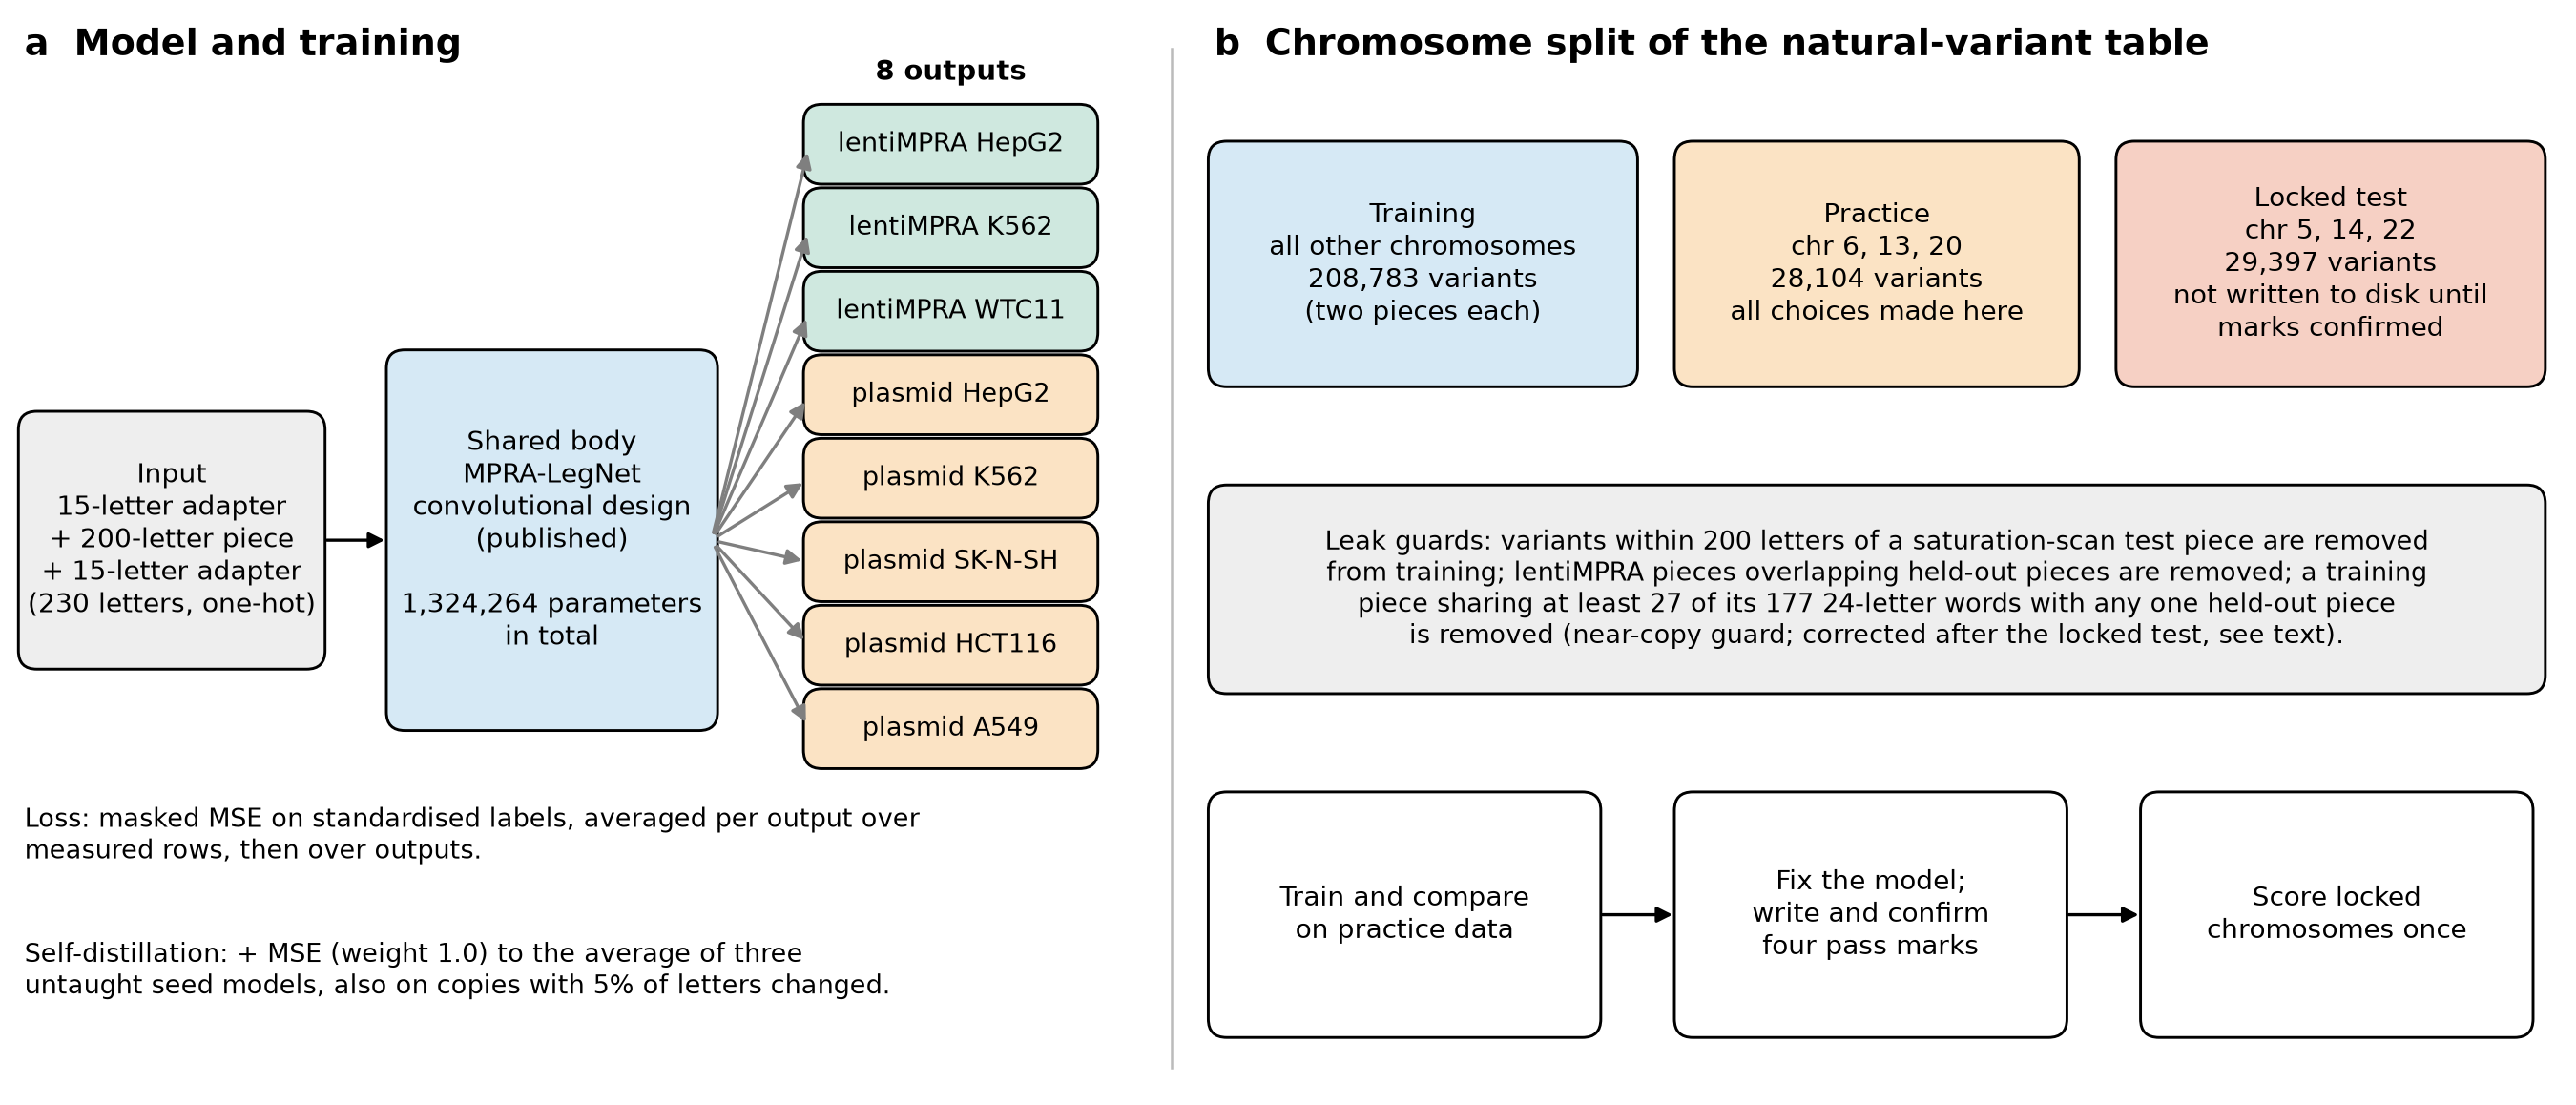
\includegraphics[width=0.94\linewidth]{figures/fig_design_and_split_schematic.png}
\caption{Model and evaluation design. (a) One MPRA-LegNet body is shared by eight outputs (three lentiMPRA and five plasmid-MPRA cell types); a masked loss trains each row only on the outputs it was measured in, and model 2 adds self-distillation. (b) The natural-variant table was split by chromosome before training; all choices were made on practice data, and the locked chromosomes were scored once after the pass marks were confirmed.}
\label{fig:schematic}
\end{figure}

\subsection{Model}
\label{sec:model}

The network is the published MPRA-LegNet design \cite{agarwal2025massively}, which uses the EfficientNetV2-inspired LegNet convolutional network \cite{penzar2023legnet,tan2021efficientnetv}, unchanged except for the output head. One shared body feeds 8 outputs: lentiMPRA HepG2, K562 and WTC11, and plasmid MPRA HepG2, K562, SK-N-SH, HCT116 and A549 (Figure~\ref{fig:schematic}a). The full model has 1,324,264 parameters (1.32M). Input is the 230-letter one-hot row; plasmid-MPRA pieces are placed between the same adapters.

Let $f_o(x)$ be output $o$ for input $x$, $y_{io}$ the standardised label of row $i$ for output $o$, and $R_o$ the set of rows in which output $o$ was measured. The label loss is a masked mean squared error, averaged per output over measured rows and then over the set of outputs $O$:
\begin{equation}
\mathcal{L}_{\text{label}} = \frac{1}{|O|}\sum_{o\in O}\frac{1}{|R_o|}\sum_{i\in R_o}\bigl(f_o(x_i)-y_{io}\bigr)^2 .
\label{eq:label}
\end{equation}
A row measured in one assay therefore trains only that assay's outputs.

\paragraph{Training recipe.} We used the published MPRA-LegNet recipe \cite{penzar2023legnet,agarwal2025massively}: 25 epochs, batch size 1024, a one-cycle learning-rate schedule \cite{smith2019superconvergence} with peak 0.01, AdamW \cite{loshchilov2017decoupled} with weight decay 0.1, random shifts of up to 21 letters filled with construct letters, and reverse-complement augmentation. The checkpoint was chosen by mean Pearson on lentiMPRA fold 9.

\paragraph{Self-distillation.} Following knowledge distillation \cite{hinton2015distilling} with a teacher of the same architecture as the student \cite{furlanello2018born}, three untaught models (same design and data, no distillation term) were first trained with different seeds. The student (model 2) was then trained on
\begin{equation}
\mathcal{L} = \mathcal{L}_{\text{label}} + \lambda\,\mathrm{MSE}\bigl(f(x), \bar{t}(x)\bigr), \qquad \lambda = 1.0,
\label{eq:distill}
\end{equation}
where $\bar{t}(x)$ is the average of the three teachers' outputs. The distillation term is applied to the training pieces and to copies of them with 5\% of letters randomly changed. Two students were trained with seeds 20261113 and 2; the first was fixed as the reported model before the locked test.

\paragraph{Variant effect.} The predicted effect of a variant is the predicted activity of the alternative version minus that of the reference version, $\hat{\Delta} = f_o(x_{\text{alt}}) - f_o(x_{\text{ref}})$. Predictions average both orientations of the insert and both strands.

\subsection{Pre-declared evaluation}
\label{sec:eval}

\paragraph{Primary metric.} Effect Pearson is the Pearson correlation between $\hat{\Delta}$ and measured log2 allelic skew on active variants (the larger of the two allele log2FC values at least 1), computed separately for HepG2 and K562 and averaged. On the locked chromosomes, 5,800 active variants were scored in HepG2 and 6,081 in K562. 95\% intervals come from 2,000 bootstrap resamples of 100,000-letter genome blocks \cite{kunsch1989jackknife} (2,580 blocks on the locked chromosomes); differences between models are computed on the same resamples. Secondary metrics are effect Spearman, activity Pearson, element Pearson on lentiMPRA, per-background Pearson on saturation scans and TraitGym AUPRC.

\paragraph{Pass marks.} The following marks were written and confirmed before the locked chromosomes were written to disk: (1) the 95\% interval of model 2 minus model 1 lies above zero; (2) the gain is at least 0.06; (3) neither HepG2 nor K562 is more than 0.01 below model 1; (4) the two seeds' means differ by at most 0.02. The locked test was run once.

\paragraph{Comparators.} \emph{Model 1} has the same design, shared body and self-distillation, but was trained on lentiMPRA only. The \emph{published MPRA-LegNet} \cite{agarwal2025massively} is the released set of single-cell-type networks (1.32M parameters, trained on lentiMPRA). The \emph{6-mer ridge} baseline is a ridge regression on 6-letter-word (6-mer) features of the sequence. \emph{MPAC} \cite{butts2025identifying} is the released ensemble of Malinois networks \cite{gosai2024machineguided} (4.1M parameters each); for each test chromosome we averaged only the 10 networks of the fold that never saw it (about 41M parameters). We ran MPAC with one centred window, the 200-letter piece padded to 600 letters with the published vector flanks, on both strands, instead of the 18 shifted windows used by its authors. Its activity Pearson here was 0.825. For every model, effects were computed as alternative minus reference and scored with the same metric and resamples.

\section{Results}
\label{sec:results}

\subsection{Blind locked test}
\label{sec:locked}

Model 2 passed all four pre-declared marks (Table~\ref{tab:locked}, Figure~\ref{fig:locked}). Its mean effect Pearson was 0.594, against 0.508 for model 1: a gain of 0.086 (95\% interval 0.074 to 0.099; mark 0.06), with HepG2 +0.089 and K562 +0.083 over model 1 and a seed gap of 0.001. It was 0.128 ahead of the published MPRA-LegNet (Table~\ref{tab:diffs}). The gain over model 1 and the published MPRA-LegNet is partly a same-assay advantage: model 2 was trained on plasmid MPRA, the assay of the test, while those two models never saw it.

Model 2 was slightly but significantly behind MPAC: $-0.010$ (95\% interval $-0.019$ to $-0.001$). The deficit was concentrated in K562 (0.555 against 0.575; HepG2 0.632 against 0.633) and was larger in Spearman (0.512 against 0.542) and activity Pearson (0.796 against 0.825). MPAC was trained on the same assay family, and our one-window run may understate it.

\begin{table}[tbp]
\centering
\caption{Blind locked test on chromosomes 5, 14 and 22 (29,397 variants). Effect Pearson on active variants (HepG2, K562, mean with 95\% block-bootstrap interval), mean effect Spearman and mean activity Pearson; higher is better. MPAC averages the 10 networks that never saw each chromosome.}
\label{tab:locked}
\footnotesize
\setlength{\tabcolsep}{4pt}
\begin{tabular}{lccccccc}
\toprule
Model & Parameters & HepG2 & K562 & Mean & 95\% interval & Spearman & Activity \\
\midrule
Model 2 (seed 20261113) & 1.32M & 0.632 & 0.555 & 0.594 & 0.566 to 0.619 & 0.512 & 0.796 \\
Model 2 (seed 2) & 1.32M & 0.630 & 0.555 & 0.592 & 0.565 to 0.618 & 0.517 & 0.798 \\
MPAC & about 41M & 0.633 & 0.575 & 0.604 & 0.578 to 0.631 & 0.542 & 0.825 \\
Model 1 & 1.32M & 0.543 & 0.472 & 0.508 & 0.479 to 0.535 & 0.406 & 0.619 \\
Published MPRA-LegNet & 1.32M & 0.487 & 0.444 & 0.466 & 0.437 to 0.493 & 0.363 & 0.590 \\
6-mer ridge baseline & -- & 0.349 & 0.290 & 0.319 & 0.293 to 0.344 & 0.283 & 0.414 \\
\bottomrule
\end{tabular}
\end{table}

\begin{figure}[htbp]
\centering
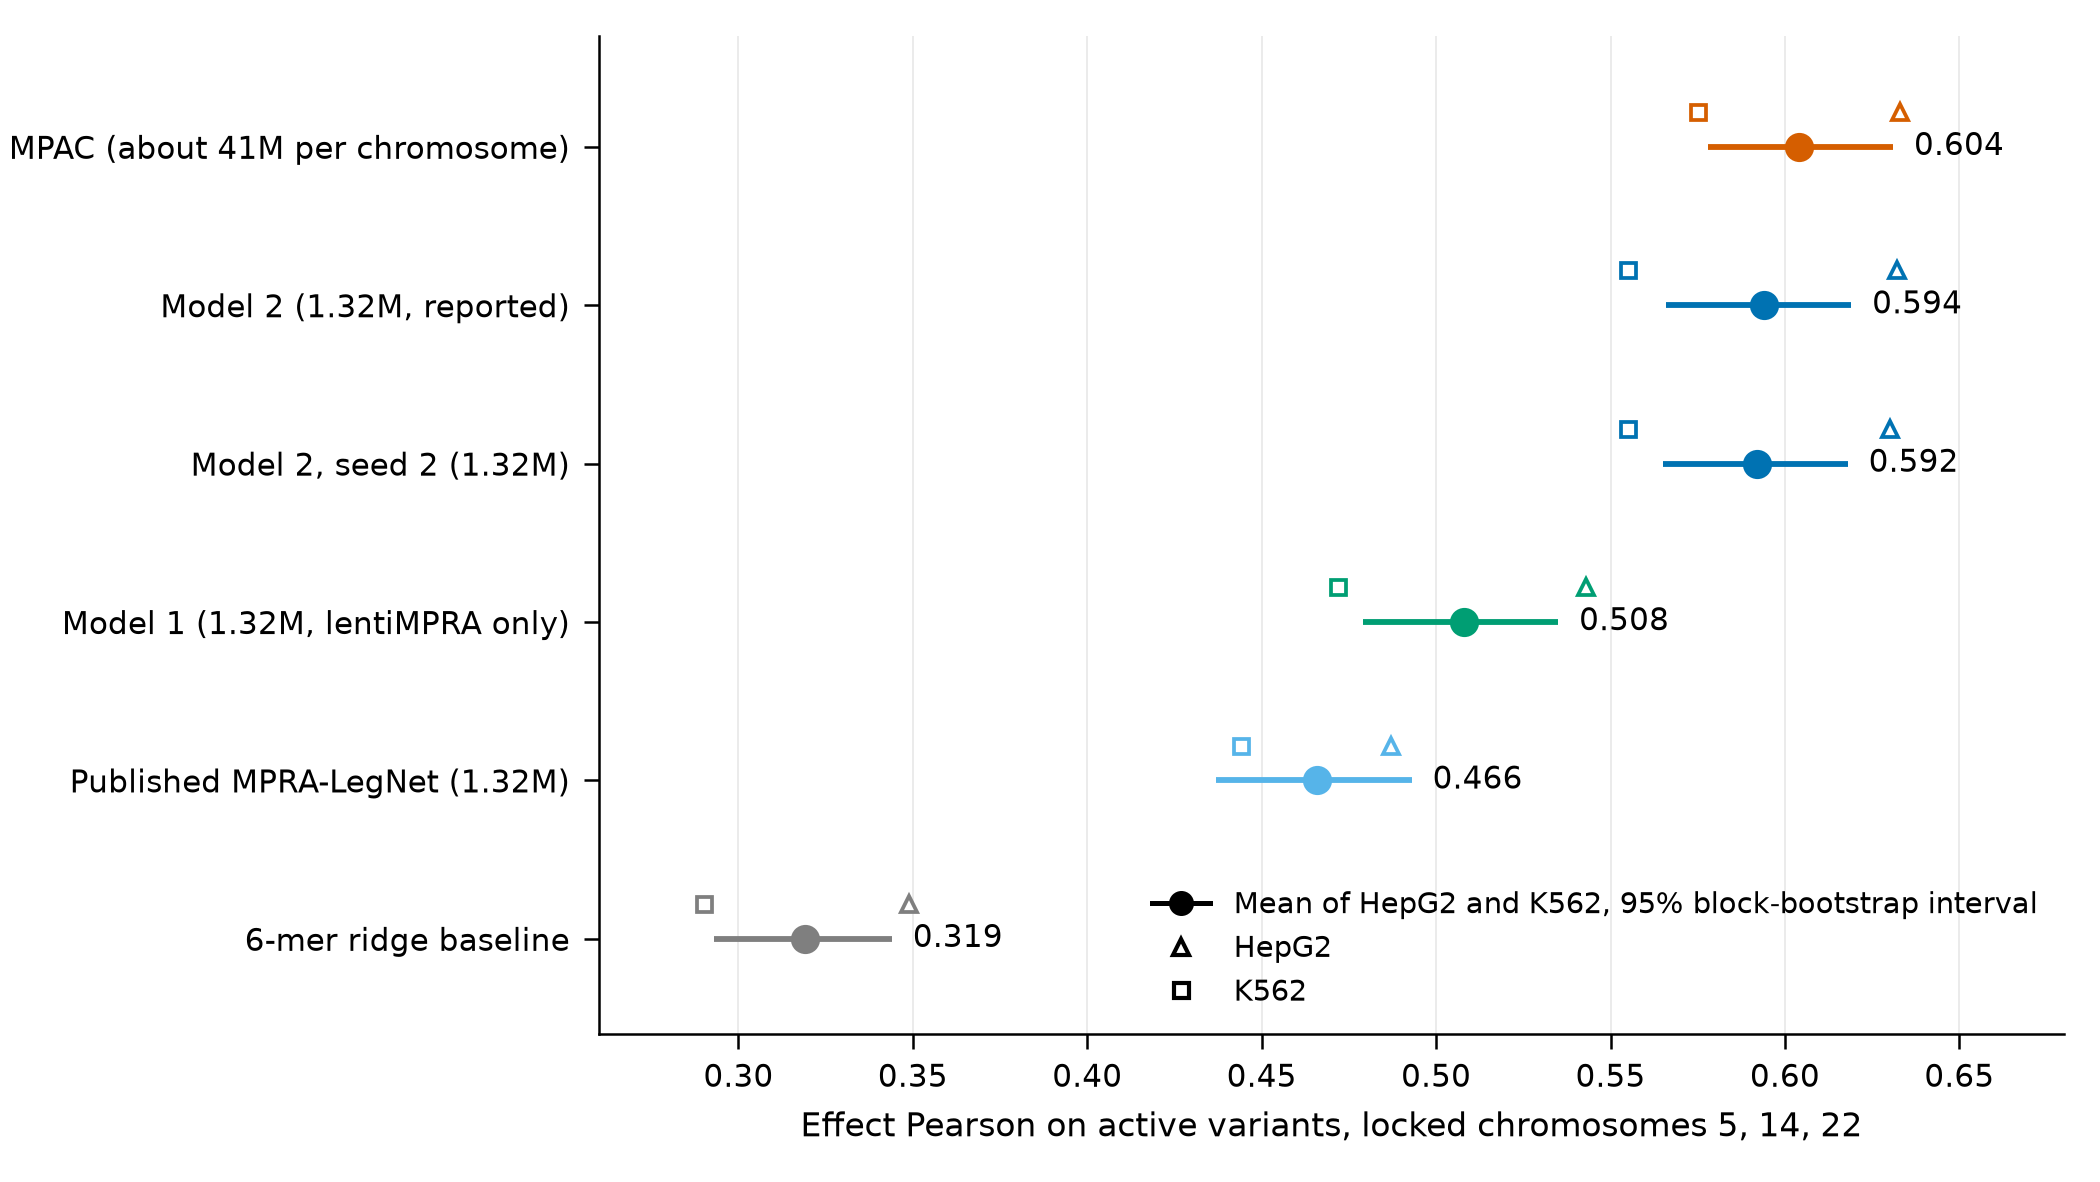
\includegraphics[width=0.66\linewidth]{figures/fig_locked_test_effect_pearson.png}
\caption{Blind locked-test results on chromosomes 5, 14 and 22. Filled circles: mean effect Pearson over HepG2 and K562 with 95\% block-bootstrap intervals; open triangles and squares: HepG2 and K562. MPAC was run with one centred window.}
\label{fig:locked}
\end{figure}

\begin{table}[tbp]
\centering
\caption{Locked test: paired differences in mean effect Pearson, computed on the same block-bootstrap resamples. Positive values favour the first model.}
\label{tab:diffs}
\small
\begin{tabular}{lcc}
\toprule
Comparison & Difference & 95\% interval \\
\midrule
Model 2 minus model 1 & 0.086 & 0.074 to 0.099 \\
Model 2 minus published MPRA-LegNet & 0.128 & 0.114 to 0.143 \\
Model 2 minus 6-mer baseline & 0.274 & 0.253 to 0.297 \\
Model 2 minus MPAC & $-0.010$ & $-0.019$ to $-0.001$ \\
Model 2 seed 20261113 minus seed 2 & 0.001 & $-0.002$ to 0.005 \\
\bottomrule
\end{tabular}
\end{table}

On variants whose pieces share no 24-letter word with any training piece, the ordering was unchanged (model 2 0.565, model 1 0.485, published MPRA-LegNet 0.443, MPAC 0.574). The SK-N-SH output, which has no counterpart in model 1, scored 0.568 on 5,935 active variants.

\subsection{Leak-guard correction}
\label{sec:leak}

After the locked test we found that our first near-copy guard looked at only the first 8 owners of each 24-letter word, so some near-copies from repeat families stayed in training: about 5.3\% of training pieces had a near-copy among practice pieces and about 5.6\% among locked pieces, and 3,277 of 29,397 locked variants had a near-copy in training. Under a rule approved before the re-score, we re-scored once without these variants (Table~\ref{tab:leak}). Model 2 moved from 0.594 to 0.590, and its gain over model 1 from 0.086 to 0.080 (95\% interval 0.068 to 0.094); all four marks still passed. On practice chromosomes the same correction moved model 2 from 0.584 to 0.577. MPAC was not re-scored on this subset, so the MPAC comparison in Section~\ref{sec:locked} uses all locked variants.

\begin{table}[tbp]
\centering
\caption{Leak-guard correction on the locked chromosomes. Mean effect Pearson over HepG2 and K562; higher is better. Without near-copies, 5,259 HepG2 and 5,389 K562 active variants remain.}
\label{tab:leak}
\footnotesize
\begin{tabular}{lccccc}
\toprule
Subset & Model 2 & Model 2 (seed 2) & Model 1 & MPRA-LegNet & 6-mer \\
\midrule
All locked variants & 0.594 & 0.592 & 0.508 & 0.466 & 0.319 \\
Without near-copies & 0.590 & 0.588 & 0.509 & 0.468 & 0.319 \\
Near-copies only & 0.627 & -- & 0.494 & 0.464 & 0.323 \\
\bottomrule
\end{tabular}
\end{table}

\subsection{Additional tests that are not blind}
\label{sec:extra}

The following sets had been read before, so these results are not blind; no choice was made from them (Table~\ref{tab:extra} in the Appendix). On the saturation-scan locked half (its second read; the first was for model 1), model 2 reached a per-background Pearson of 0.718 against 0.625 for model 1 (interval of the difference 0.071 to 0.116) and 0.588 for the published MPRA-LegNet. This set comes from the same plasmid MPRA study as model 2's added training data. On the four elements of \citet{kircher2019saturation}, model 2 reached 0.656 against 0.639 for model 1 (interval 0.000 to 0.033), better on F9 and PKLR and worse on LDLR and SORT1. On lentiMPRA fold 10, model 2 scored 0.837 against 0.842 for model 1 (interval $-0.008$ to $-0.001$), slightly but significantly lower, mostly in K562, while adding five plasmid-MPRA outputs; both remain above the published MPRA-LegNet (0.818).



\paragraph{Out-of-scope check.} Model 2 is not a disease-variant scorer. On TraitGym Mendelian it reached a pooled AUPRC of 0.259 (95\% interval 0.218 to 0.308; random is about 0.10), against 0.267 for model 1, 0.296 for PhyloGPN and 0.694 for CADD.

\subsection{What closes the gap: training method}
\label{sec:ablation}

On practice chromosomes, most of model 2's gain over model 1 (0.491) came from adding plasmid-MPRA data to the shared body: three seeds without self-distillation all scored 0.573. Self-distillation raised this to 0.584 in both seeds (about 0.011), with similar small gains on the saturation-scan practice half and lentiMPRA fold 9 (Table~\ref{tab:ablation} in the Appendix).



\subsection{Where the gap to MPAC comes from}
\label{sec:decomp}

Without further training, we compared single MPAC networks and averages of networks on the practice chromosomes (Figure~\ref{fig:decomp}; Table~\ref{tab:decomp} in the Appendix). Single MPAC networks scored 0.578 to 0.588 (mean 0.583), the same as model 2 (0.584), while averaging 2, 3, 5 and 10 MPAC networks gave 0.601, 0.604, 0.608 and 0.609. Averaging our own models gained much less (0.589 for all 10), adding model 2 to the MPAC average gave 0.608, and test-time shift averaging added only 0.002 to model 2. The mean pairwise Pearson of predicted effects was 0.908 between MPAC networks and 0.958 between our seeds. The ensemble's lead therefore comes from averaging, not from a better single network, and goes with lower agreement between its members. MPAC's members differ in held-out folds and in their training recipe; we did not test which of these makes them less alike, or whether lower agreement causes the larger gain.

\begin{figure}[htbp]
\centering
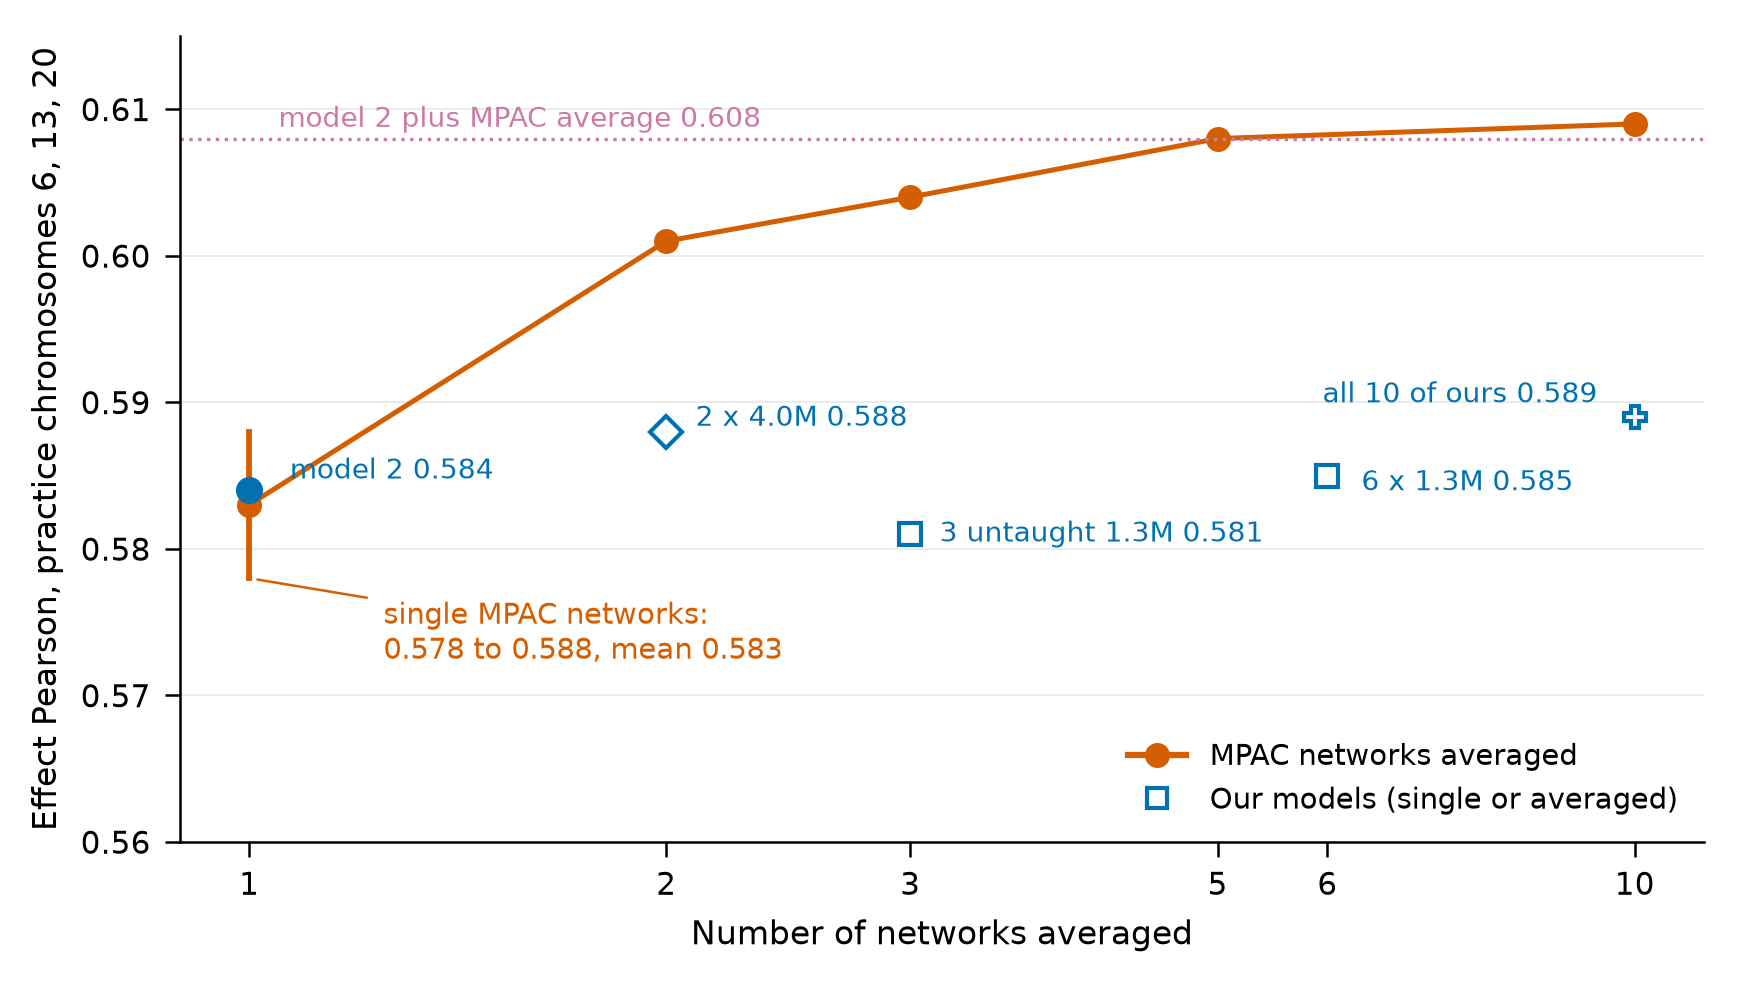
\includegraphics[width=0.58\linewidth]{figures/fig_ensemble_gap_decomposition.png}
\caption{Where the gap to MPAC comes from, on practice chromosomes 6, 13 and 20 (no training). Single MPAC networks are about as accurate as model 2; averaging MPAC networks gains more than averaging our own models.}
\label{fig:decomp}
\end{figure}

\subsection{Changes that did not help}
\label{sec:negative}

We screened one change at a time on practice data against model 2 without self-distillation (0.573; Figure~\ref{fig:screen}; full values in Table~\ref{tab:screen} in the Appendix). Only a wider body helped: 4.0M parameters gave 0.582 (+0.009 with 3 times the parameters). An extra loss on the difference between the two versions of a variant hurt (0.560 and 0.554); a control with the same paired batches and negligible loss weight scored 0.578, so the loss term was the harmful part. About 142,000 extra pieces from the larger table of the same assay gave 0.575 in both seeds, and EvoAug-style augmentation \cite{lee2023evoaug} hurt (0.545 to 0.558). The Malinois design \cite{gosai2024machineguided} (5.0M parameters) trained with our recipe scored 0.472 and 0.484, and 0.521 with peak learning rate 0.003; these runs were still improving at the last epoch, so they were undertrained and say little about the design itself. Dropping noisy pieces (maximum standard error 1.0) gave 0.575 and duplicating active pieces 0.572. An earlier design screen on model 1 also found no gain (Appendix).

\begin{figure}[htbp]
\centering
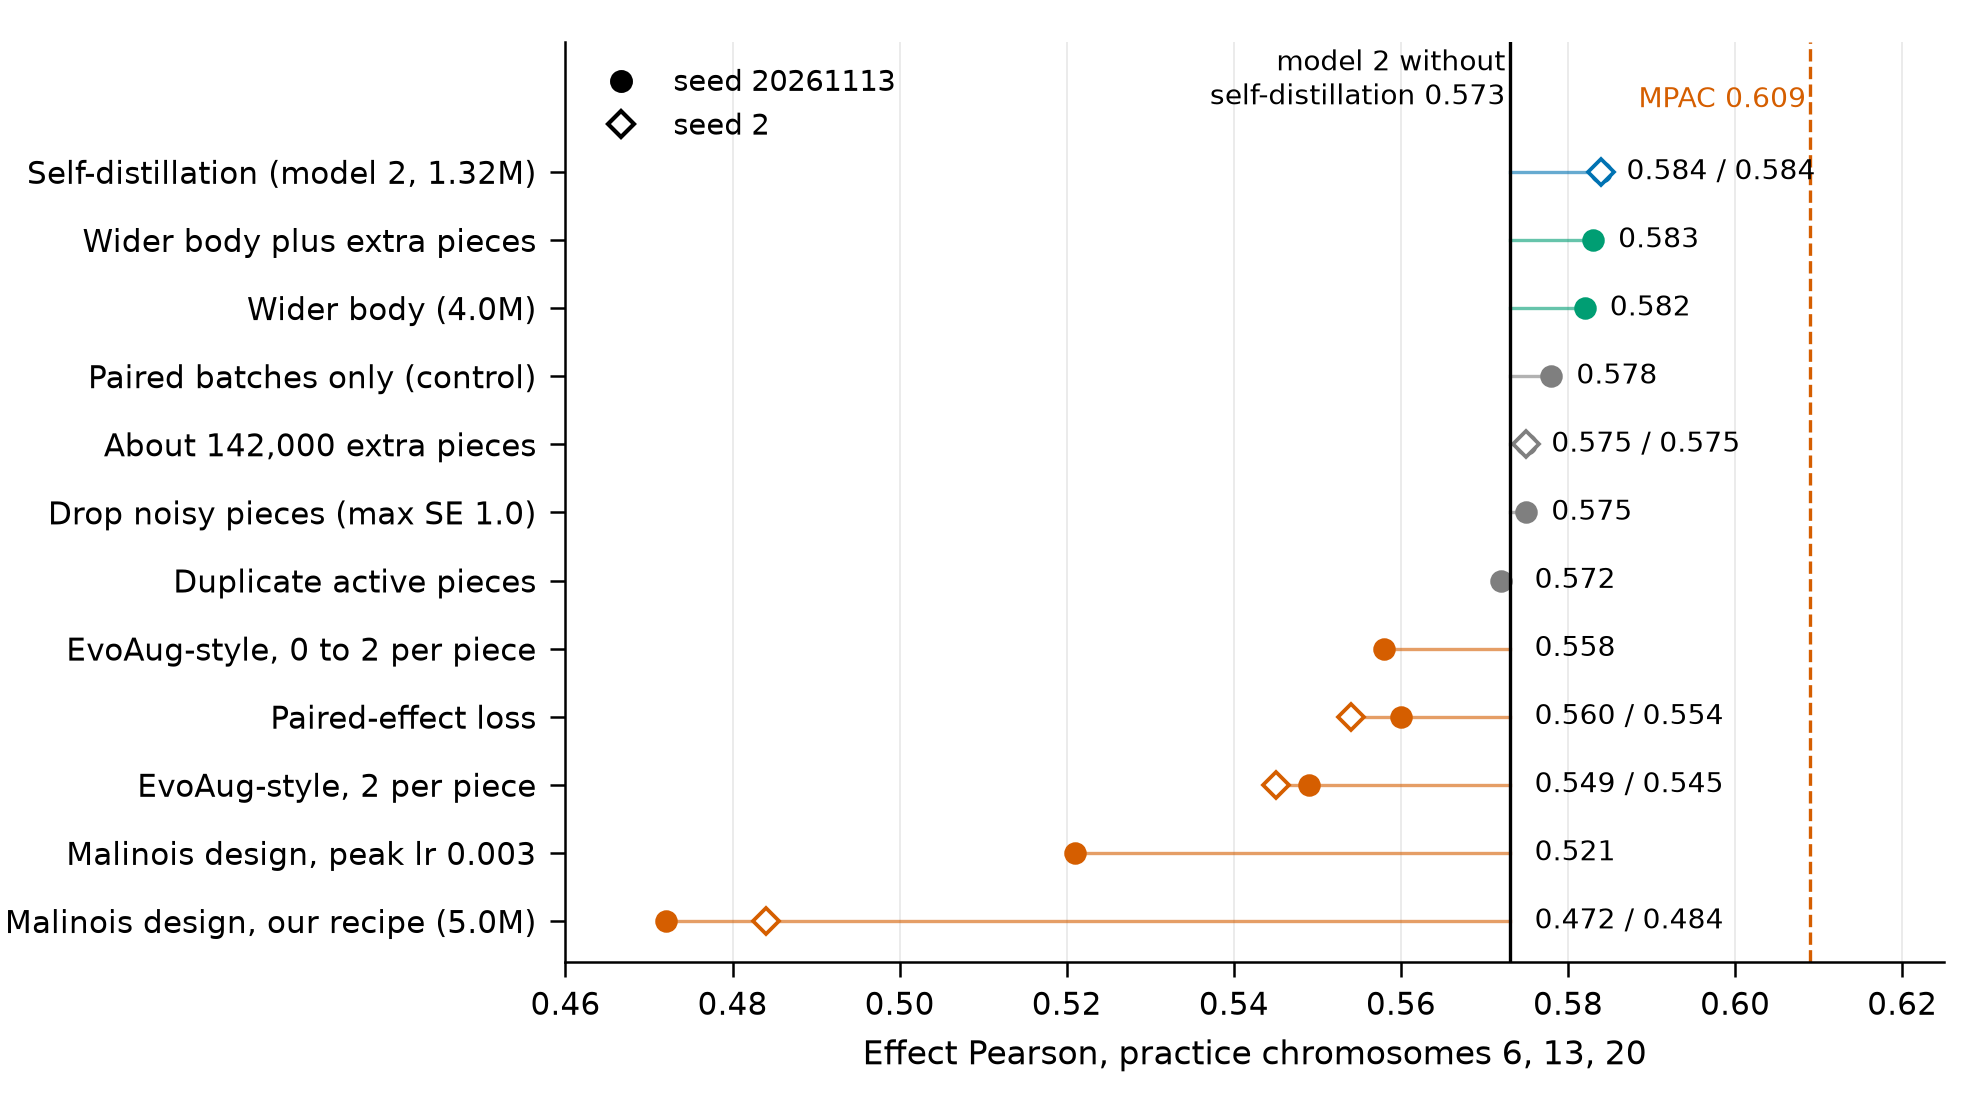
\includegraphics[width=0.66\linewidth]{figures/fig_practice_screen_changes.png}
\caption{One-change screens on practice chromosomes against model 2 without self-distillation (black line); dashed line: 10-network MPAC average. Circles and diamonds: two seeds.}
\label{fig:screen}
\end{figure}

\section{Discussion and Limitations}
\label{sec:discussion}

\paragraph{What the results show.} Adding same-assay data through a shared multi-assay body brought a single network with the published MPRA-LegNet design within 0.010 of the MPAC ensemble on blind chromosomes, slightly but significantly behind it. Model 2 is about 3 times smaller than one comparable single network (1.32M against 4.1M parameters) and about 31 times smaller than the ensemble used for each chromosome (about 41M); we did not measure inference speed or cost. Because a single MPAC network is no more accurate than model 2, the remaining gap is an ensembling effect; distilling a more diverse set of members into one small network is an untested next step. The design and recipe are published; our additions are the shared body, self-distillation (a small gain), the protocol, the decomposition and the negative results. Since the largest gain came from data of the test's assay type, the gain over model 1 and the published MPRA-LegNet is partly a same-assay advantage, and the fair comparator is MPAC, which was also trained on this assay family.

\paragraph{Limitations.} (i) MPAC was run with one centred window instead of 18 shifted windows, which may understate it, so the true gap may be larger than 0.010. (ii) The near-copy guard was flawed in the locked test; the disclosed re-score changed the main result by 0.004 and no verdict, but MPAC was not re-scored on the clean subset. (iii) The additional tests are not blind. (iv) Label noise bounds attainable correlation: estimated reliability of single-letter effects among active pieces is 0.83 to 0.87. (v) The evaluation uses one natural-variant table, one chromosome split and two cell types for the primary metric. (vi) All data come from plasmid and lentiviral MPRAs in cancer and stem-cell lines; episomal and integrated reporters can differ from endogenous chromatin \cite{inoue2016systematic}, so results may not transfer to endogenous genomic context.

\section{Conclusion}
\label{sec:conclusion}

One 1.32M-parameter network trained across two MPRA assay families predicted single-letter allelic skew on blind chromosomes at an effect Pearson of 0.594, far ahead of the published small model and slightly but significantly behind a 10-network ensemble (difference $-0.010$). A single member of that ensemble was no better than our network, so the ensemble's advantage comes from averaging; whether it can be distilled into one small network remains open.

\section*{Data and Code Availability}

All data \cite{agarwal2025massively,siraj2026functional,kircher2019saturation,benegas2025benchmarking} and comparator weights \cite{agarwal2025massively,butts2025identifying} are available from the original publications. Training, evaluation and leak-guard code, the pre-declaration with the pass marks, the weights of both model 2 seeds and a prediction script will be released; model 1 and model 2 will be released as Cislume Lohit and Cislume Dibang. Because the natural-variant data used to train model 2 are licensed for non-commercial use only (CC BY-NC) \cite{siraj2026functional}, model 2's weights will be released under a non-commercial licence. [Repository URL to be added by the authors.]

\bibliographystyle{unsrtnat}
\bibliography{refs}

\clearpage
\appendix
\section{Additional tables}
\label{sec:appendix}

\begin{table}[h]
\centering
\caption{Practice data: effect of the training method. Practice chromosomes and scan practice half: mean effect Pearson over HepG2 and K562; fold 9: lentiMPRA element Pearson. Higher is better.}
\label{tab:ablation}
\footnotesize
\begin{tabular}{lccc}
\toprule
Model & Practice chromosomes & Scan practice half & LentiMPRA fold 9 \\
\midrule
Model 1 (lentiMPRA only) & 0.491 & 0.627 & 0.842 \\
Published MPRA-LegNet & 0.455 & 0.579 & 0.816 \\
6-mer baseline & 0.313 & 0.382 & -- \\
Model 2 without self-distillation (3 seeds) & 0.573 & 0.679 to 0.687 & 0.829 to 0.833 \\
Model 2 with self-distillation (2 seeds) & 0.584 / 0.584 & 0.699 / 0.696 & 0.844 / 0.840 \\
\bottomrule
\end{tabular}
\end{table}

\begin{table}[h]
\centering
\caption{One-change screens on practice data, against model 2 without self-distillation (practice chromosomes 0.573; scan practice half 0.679 to 0.687; lentiMPRA fold 9 0.829 to 0.833). Values for two seeds are separated by a slash. Higher is better.}
\label{tab:screen}
\footnotesize
\begin{tabular}{p{6.4cm}ccc}
\toprule
Change & Practice chromosomes & Scan practice half & LentiMPRA fold 9 \\
\midrule
Extra loss on the difference between the two versions (2 seeds) & 0.560 / 0.554 & 0.666 / 0.670 & 0.808 \\
Same paired batches, negligible loss weight (control) & 0.578 & 0.684 & -- \\
About 142,000 extra same-assay pieces (2 seeds) & 0.575 / 0.575 & 0.688 / 0.697 & -- \\
Wider body, 4.0M parameters & 0.582 & 0.694 & 0.838 \\
Wider body plus extra pieces & 0.583 & 0.704 & 0.840 \\
EvoAug-style augmentation, 2 per piece, then 5 clean epochs (2 seeds) & 0.549 / 0.545 & 0.653 / 0.652 & 0.808 / 0.804 \\
EvoAug-style augmentation, 0 to 2 per piece & 0.558 & 0.666 & 0.821 \\
Malinois design, 5.0M parameters, our recipe (2 seeds) & 0.472 / 0.484 & 0.580 / 0.580 & 0.755 / 0.758 \\
Malinois design, peak learning rate 0.003 & 0.521 & 0.598 & 0.790 \\
Drop pieces with max standard error 1.0 & 0.575 & 0.683 & 0.831 \\
Duplicate active pieces (log2FC at least 0.5) & 0.572 & 0.679 & 0.832 \\
\bottomrule
\end{tabular}
\end{table}

Earlier design screen on the lentiMPRA-only model (lentiMPRA fold 9 mean / scan practice half), against 0.833 / 0.614: per-cell-type heads 0.835 / 0.609; no pooling after the first block 0.834 / 0.598; strand-symmetric network 0.821 / 0.569; weight averaging (EMA) 0.829 on fold 9 (scan not scored).

\begin{table}[h]
\centering
\caption{Additional tests on sets that had been read before (not blind). Saturation scans: per-background Pearson; lentiMPRA fold 10: element Pearson. Higher is better.}
\label{tab:extra}
\footnotesize
\begin{tabular}{lcccc}
\toprule
Test & Model 2 & Model 1 & MPRA-LegNet & 6-mer \\
\midrule
Saturation scan, locked half (mean of HepG2, K562) & 0.718 & 0.625 & 0.588 & 0.386 \\
\quad HepG2 & 0.693 & -- & -- & -- \\
\quad K562 & 0.742 & -- & -- & -- \\
Four-element saturation mutagenesis, mean & 0.656 & 0.639 & 0.594 & -- \\
\quad F9 & 0.724 & 0.582 & -- & -- \\
\quad LDLR & 0.564 & 0.637 & -- & -- \\
\quad SORT1 & 0.565 & 0.645 & -- & -- \\
\quad PKLR (48 hours) & 0.770 & 0.693 & -- & -- \\
LentiMPRA fold 10, mean of three cell types & 0.837 & 0.842 & 0.818 & -- \\
\quad HepG2 & 0.842 & 0.841 & 0.818 & -- \\
\quad K562 & 0.856 & 0.868 & 0.857 & -- \\
\quad WTC11 & 0.813 & 0.816 & 0.779 & -- \\
\bottomrule
\end{tabular}
\end{table}

\begin{table}[h]
\centering
\caption{Practice chromosomes: single networks and averages (no training). Higher is better.}
\label{tab:decomp}
\small
\begin{tabular}{lc}
\toprule
Predictor & Effect Pearson \\
\midrule
Single MPAC networks (10 networks) & 0.578 to 0.588, mean 0.583 \\
Average of 2 / 3 / 5 / 10 MPAC networks & 0.601 / 0.604 / 0.608 / 0.609 \\
Model 2 (single network) & 0.584 \\
Average of 3 of our untaught models & 0.581 \\
Average of 6 of our 1.3M models & 0.585 \\
Average of 2 of our 4.0M models & 0.588 \\
Average of all 10 of our models & 0.589 \\
Model 2 plus MPAC average & 0.608 \\
Model 2 with test-time shift averaging & +0.002 over model 2 \\
\midrule
Mean pairwise agreement of predicted effects: MPAC networks & 0.908 \\
Mean pairwise agreement of predicted effects: our seeds & 0.958 \\
\bottomrule
\end{tabular}
\end{table}

\end{document}
